%****************************************
% Lab 07: Timer
%****************************************
\chapter{Timer}

\section{Purpose}

A timer is used to time events. This lab creates a timer where the minimum and maximum counts can be set and counts both up and down. The timer assumes an input clock pulse at 1 Hz (or 60 pulses per minute) but for testing, the clock can be set to any value.

\section{Procedure}

The lab starter circuit includes several versions of the timer as an illustration of the thought process used to develop the final product.

\begin{itemize}
	\item \textbf{Timer\_V1}. This is little more than a test of the Counter (\textit{Memory} library) component. The various inputs were wired so both the \textit{Load} and \textit{Up} input pins could be tested. Instead of a clock pulse, a Button (\textit{Input/Output} library) was used for better control over the device. A Bin2BCD (\textit{BFH mega functions} library) device was used for easier interpretation of the output.
	\item \textbf{Timer\_V2}. The first circuit was expanded such that both the minimum and maximum counts could be specified. Note that the multiplexer (\textit{Plexers} library) selects whether the minimum or maximum number is loaded depending on whether the count is Up or Down.
	\item \textbf{Timer\_V3}. This is the version of the timer that will be completed for this lab.
\end{itemize}

\subsection{Timer\_V3}

Complete the circuit to match Figure \ref{fig:07-01}.

\begin{figure}[H]
	\centering
	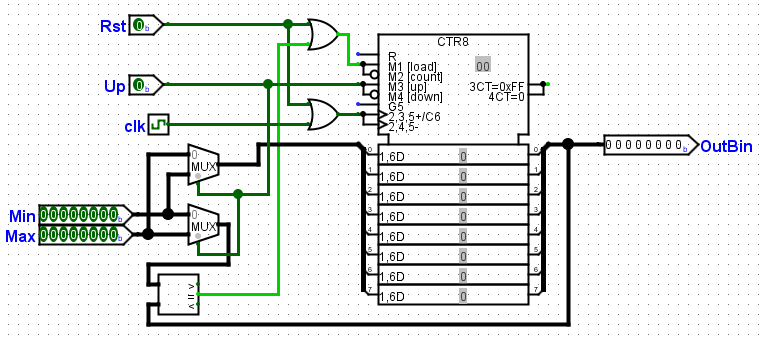
\includegraphics[width=\maxwidth{.95\linewidth}]{gfx/07-01}
	\caption{Completed Timer}
	\label{fig:07-01}
\end{figure}

In the timer circuit, the key is the comparator in the lower left corner. That device compares the binary output of the counter to either the minimum or maximum requested value and if they are equal the comparator sends a reset signal to start the count over. 

There are two multiplexers with a subtle, but important, difference. The Maximum input value is wired to the top input of the top multiplexer but the bottom input of the bottom multiplexer. The result is the when the count is ``Up'' the Minimum input is loaded into the counter but the Maximum input is used in the compare, so the counter starts at the minimum and counts up to the maximum. The opposite is true for a ``Down'' count.

Finally, the BCD output is combined by a splitter (\textit{Wiring} library) into a 12-bit bus for transmission.

\subsection{Testing the Circuit}

The \lstinline[columns=fixed]|Timer_V3| subcircuit should be added to the \lstinline[columns=fixed]|main| circuit and wired as in Figure \ref{fig:07-02}.

\begin{figure}[H]
	\centering
	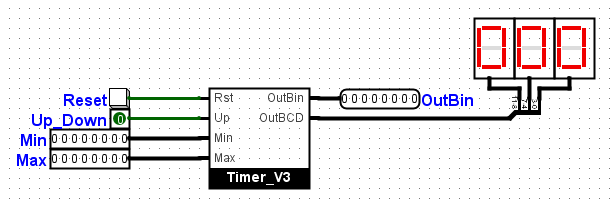
\includegraphics[width=\maxwidth{.95\linewidth}]{gfx/07-02}
	\caption{Timer Main Circuit}
	\label{fig:07-02}
\end{figure}
 
To test the circuit:

\begin{enumerate}
	\item Enter binary four for a minimum value and eight for a maximum value. (Actually, any values can be entered but four and eight are enough to test the circuit.) 
	\item Poke \textit{Up\_Down} to change its value to one so the circuit counts up.
	\item Poke the Reset button and observe that the BCD out changes to 004.
	\item Activate the clock \textsc{Simulate -> Ticks Enabled} and observe that it counts up from four to eight and then resets to four. If the speed of the timer is not reasonable then the \textsc{Simulate -> Tick Frequency} can be adjusted.
	\item Poke \textit{Up\_Down} to change the count to down and observe that the timer now counts from eight to four and resets.
\end{enumerate}

\section{Challenge}

As designed, the output of this circuit is an integer count. If it were set for counting seconds then the count of seconds would increase from 59 to 60 then 61 rather than going 0:59, 1:00, 1:01 as expected. Rewrite the \lstinline[columns=fixed]|Timer_V3| subcircuit so the output is two BCD numbers: minutes and seconds. As a hint, the Divider (\textit{Arithmetic} library) device products an integer (``modulus'') division along with a remainder. It should help to divide the count by 60, use the whole number as ``minutes'' and the remainder as the ``seconds.''

\section{Deliverable}

To receive a grade for this lab, complete the Challenge. Be sure the standard identifying information is at the top left of the \lstinline{main} circuit, similar to: 

\bigskip
% The minipage environment keeps the three lines together - no page break.
\begin{minipage}{\linewidth}
	\begin{verbatim}
	George Self
	Lab 07: Timer
	March 1, 2018
	\end{verbatim}
\end{minipage}
\bigskip

Save the file with this name: \emph{\texttt{Lab07\_Timer}} and submit that file for grading.

